\section{Parameter estimation errors}
\label{section:estimation-experiment}

The goal of the last numerical experiment is to explain the reason behind low sensitivity of MD, especially when compared with conceptually similar SED measure, e.g., visible when comparing the histograms in figures \ref{fig:hists-correlations-md} and \ref{fig:hists-correlations-sed}, also observing the rapid sensitivity decay for MD in higher dimensions $d$ in figure \ref{fig:dimension-sensitivity}. Both mentioned measures rely on estimating the vector of means $\mu$ and either the full covariance matrix $\Sigma$ or only its diagonal elements (variances). The analysis of errors impact is conducted as a function of the~feature space dimension $d$ and the~number of samples $n$.

\vspace{2.0em}  % NOTE: Just to expand the elements on page a little


\subsection{Experiment organization}
\label{section:estimation-organization}

The experiment is organized as follows:
\vspace{-0.5\baselineskip}
\begin{itemize}
    \item First, a single data cluster $K$ is generated.
          \begin{itemize}
              \item The dataset is produced from the Multivariate Normal distribution (MVN), containing $n$ samples of~dimension~$d$, located around the~center of~the coordinate system $\mu = [0, 0, \dots, 0]$ with a spread of $\pm 1$).
              \item The distribution shape is influenced by two additional parameters:
                    \begin{itemize}
                        \item the fraction of features that are correlated $f_{corr}$,
                        \item the strength of the features correlation $g_{corr}$.
                    \end{itemize}
                    These parameters affect the content of the covariance matrix $\Sigma$ supplied to the MVN generator, e.g., for $d = 5$, $f_{corr} = 0.6$ and $g_{corr} = 0.25$ it results in
                    \begin{equation}
                        \Sigma
                        =
                        \begin{bmatrix}
                            \mathbf{1.00} & \mathbf{0.25} & \mathbf{0.25} & 0.00 & 0.00 \\
                            \mathbf{0.25} & \mathbf{1.00} & \mathbf{0.25} & 0.00 & 0.00 \\
                            \mathbf{0.25} & \mathbf{0.25} & \mathbf{1.00} & 0.00 & 0.00 \\
                            0.00 & 0.00 & 0.00 & \mathbf{1.00} & 0.00 \\
                            0.00 & 0.00 & 0.00 & 0.00 & \mathbf{1.00}
                        \end{bmatrix}
                        .
                        \label{eq:corr-example-2}
                    \end{equation}
          \end{itemize}
    \item The sample mean $\hat{\mu}$ and empirical covariance $\hat{\Sigma}$ are estimated on the dataset $K$.
    \item The Mean Squared Error (MSE) of the estimates are calculated as per formula,
          \begin{equation}
              MSE(A, \hat{A})
              =
              \frac{1}{w}
              \cdot
              \sum_{i=1}^{w}
              \left(
                  A_i - \hat{A}_i
              \right)^2
              ,
              \label{eq:MSE}
          \end{equation}
          where $A$ is the true/expected value of a~parameter and $\hat{A}$ is its estimated value, $w$~is~the~number of components if $A$ is a~vector or matrix, $i$ indexes the components. In~particular, the inaccuracies of the~following parameters were computed:
          \begin{itemize}
              \item means: $MSE(\mu, \hat{\mu})$;
                    $w = d$;
              \item covariance matrices: $MSE(\Sigma, \hat{\Sigma})$;
                    $w = d^2$;
              \item variances: $MSE(\Sigma_{i,j}, \hat{\Sigma}_{i,j})$
                    where
                    $\forall (i, j) \in \{1, 2, \dots, d\}: i = j$;
                    $w = d$;
              \item correlations: $MSE(\Sigma_{i,j}, \hat{\Sigma}_{i,j})$
                    where
                    $\forall (i, j) \in \{1, 2, \dots, d\}: i \neq j$;
                    $w = \frac{d}{d - 1}$.
          \end{itemize}
\end{itemize}

Summarizing, the input parameters that vary in the experiment are: the number of~samples $n$, dimension of the feature space $d$, the fraction of~features that are correlated $f_{corr}$ and the strength of the correlation $g_{corr}$. The experiment was repeated several times with various values of the generator seed $\xi$.


\subsection{Experiment results}
\label{section:estimation-results}

The fifth experiment is a numerical study of how accurate the empirical estimations of distribution properties are, considering number of samples in cluster $n$ and the dimension $d$ of vectors, focusing in the high-dimensional feature spaces in particular.

Figure \ref{fig:estimation} presents the results obtained for a Multi-variate Normal (MVN) distribution with small fraction of features $f_{corr} = 0.2$ slightly correlated $g_{corr} = 0.2$. The experiment is conducted for a range of correlation settings and the results do not differ significantly – unless a very strong correlation of features in data is involved (as shown in the figure \ref{fig:estimation-strong}.

Surprisingly, all three analyzed parameters: means, variances and covariances; are estimated with similar accuracy for a given experiment configuration ($n$, $d$, $f_{corr}$, $g_{corr}$). The estimation errors are primarily related to the number of available data samples $n$, with the behavior being inversely proportional – the more examples provided, the lesser error (more accurate representation of the original/expected values). The estimation accuracy appears not significantly affected by the dimensionality of the feature space.

Comparing the results side-by-side (figures \ref{fig:estimation-means}, \ref{fig:estimation-variances} and \ref{fig:estimation-covariances}) it can be noticed that the estimation errors for means and covariances appear nearly the same, especially for higher dimensionality ($d \geq 100$), while the estimation of variances appear slightly worse (higher error). However, all estimation errors for a given set of parameters ($n$, $d$, $f_{corr}$, $g_{corr}$) are of the same order of magnitude.

\clearpage  % NOTE: To avoid splitting the list between pages

\begin{itemize}
    \item $d = 1000$, $f_{corr} = 0.2$, $g_{corr} = 0.2$, $n = 1000$:
          \begin{itemize}
              \item $MSE( \text{means} ) \approx 1.0 \cdot 10^{-3}$,
              \item $MSE( \text{variances} ) \approx 0.9 \cdot 10^{-3}$,
              \item $MSE( \text{covariances} ) \approx 1.0 \cdot 10^{-3}$;
          \end{itemize}
    \item $d = 1000$, $f_{corr} = 0.2$, $g_{corr} = 0.2$, $n = 10000$:
          \begin{itemize}
              \item $MSE( \text{means} ) \approx 1.0 \cdot 10^{-4}$,
              \item $MSE( \text{variances} ) \approx 0.9 \cdot 10^{-4}$,
              \item $MSE( \text{covariances} ) \approx 1.0 \cdot 10^{-4}$.
          \end{itemize}
\end{itemize}

This observation is significant, because when considering how the computed values are involved in the distances calculation for the MD measure (section \ref{section:Mahalanobis}, formula \ref{eq:md}) or the SED measure (section \ref{section:SEuclidean}, formula \ref{eq:sed}), the various cumulative error can be estimated. Assuming the average estimation error of a single parameter, e.g., the variance on the $j$-th axis or the covariance between features $j_1$ and $j_2$ (element $\Sigma_{j_1,j_2}$), being $\delta$ in both cases (same order of magnitude), when computing the Standardized Euclidean distance, each of the $d$ estimated variances scales the corresponding distances (vector components) that are later summed up, leading to a total cumulative error
\begin{equation}
    Err( \text{SED} )
    \approx
    \underbrace{
        \vphantom{\frac{a}{b}}  % Spacing hack – moves the underbrace a little down
        \delta + \delta + \dots + \delta
    }_{d~\text{components}}
    = d \cdot \delta
    \quad
    \sim
    \order{ d },
    \label{eq:sed-error}
\end{equation}
while the Mahalanobis distance formula (matrix times vector) involves $d$ multiplications and additions for each of the $d$ vector components, leading to a total cumulative error
\begin{equation}
    Err( \text{MD} )
    \approx
    \underbrace{
        \vphantom{\frac{a}{b}}  % Spacing hack – moves the underbrace a little down
        d \cdot \delta + d \cdot \delta + \dots + d \cdot \delta
    }_{d~\text{components}}
    = d^2 \cdot \delta
    \quad
    \sim
    \order{ d^2 }.
    \label{eq:md-error}
\end{equation}

Hence, summarizing, as long as no significant correlation of feature is involved, the SED appears to~be preferable than MD, promising more accurate distance calculation in high-dimensional feature spaces.

The obtained results justifies why it is worth to increase the number of training samples $n$ for the estimation of covariance matrix $\Sigma$, and hence the utilization of pooled covariance matrix is motivated, i.e., single common covariance matrix assumed for all in-distribution classes (MDP measure, section \ref{section:Mahalanobis}). However, as it is shown in next chapter, the latter mentioned approach suffers also from the other kind of method error.

\begin{figure}[t]
    % StreamLit settings: width=9, height=4
    % X: [0.95, 10500.00]
    % Y: [0,000005, 1.20]
    \centering
    \vspace{-0.5em}
    \begin{subfigure}[b]{0.9\textwidth}
        \centering
        \caption{\small Error estimating means}
        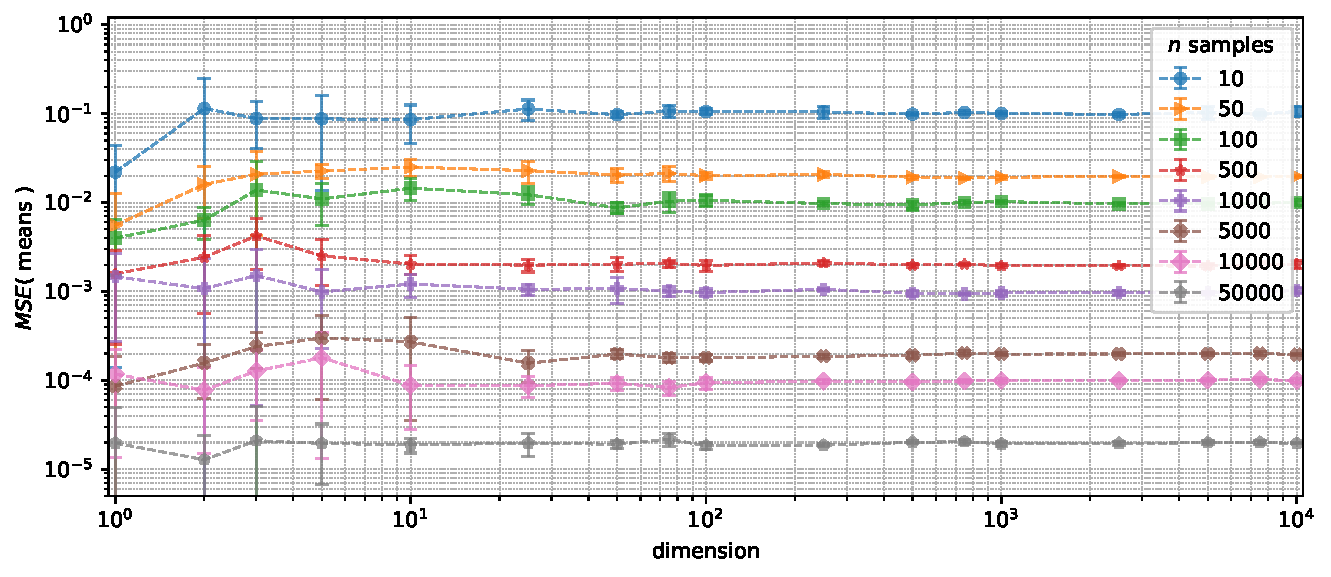
\includegraphics[width=\textwidth]{images/estimation/trend-properties-mse_means(dimension)-n_correlated_0.20-covariance_0.20-samples_10,50,100,500,1000,5000,10000,50000-aggregated.pdf}
        \label{fig:estimation-means}
    \end{subfigure}

    \vspace{-0.5em}
    \begin{subfigure}[b]{0.9\textwidth}
        \centering
        \caption{\small Error estimating variances}
        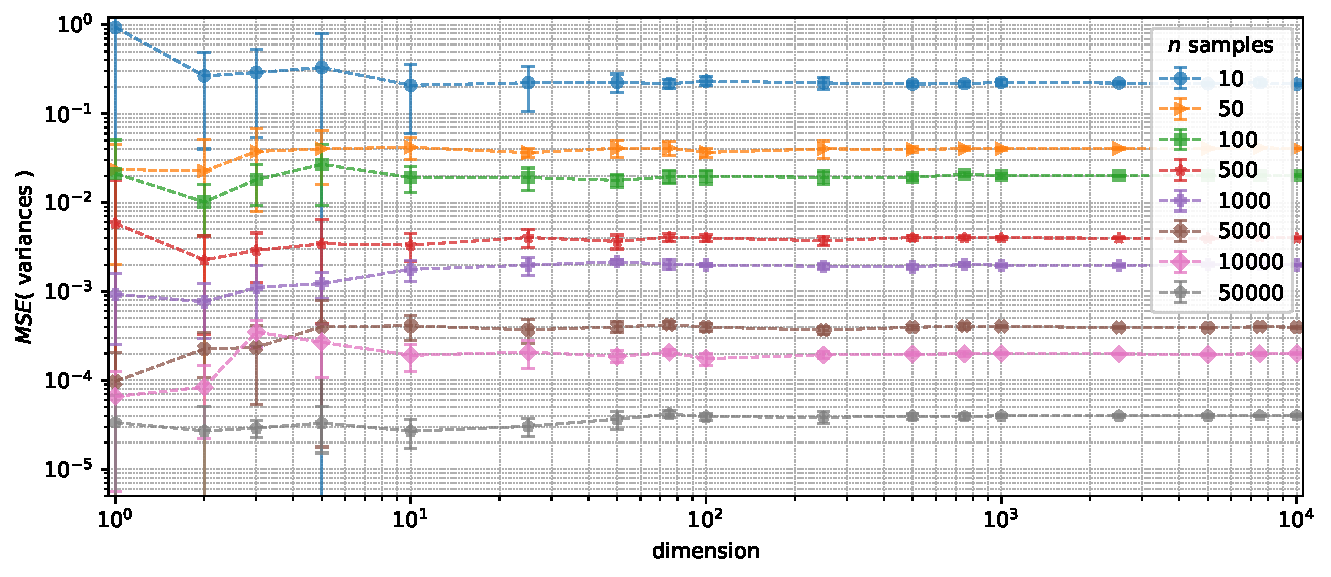
\includegraphics[width=\textwidth]{images/estimation/trend-properties-mse_vars(dimension)-n_correlated_0.20-covariance_0.20-samples_10,50,100,500,1000,5000,10000,50000-aggregated.pdf}
        \label{fig:estimation-variances}
    \end{subfigure}

    \vspace{-0.5em}
    \begin{subfigure}[b]{0.9\textwidth}
        \centering
        \caption{\small Error estimating covariances}
        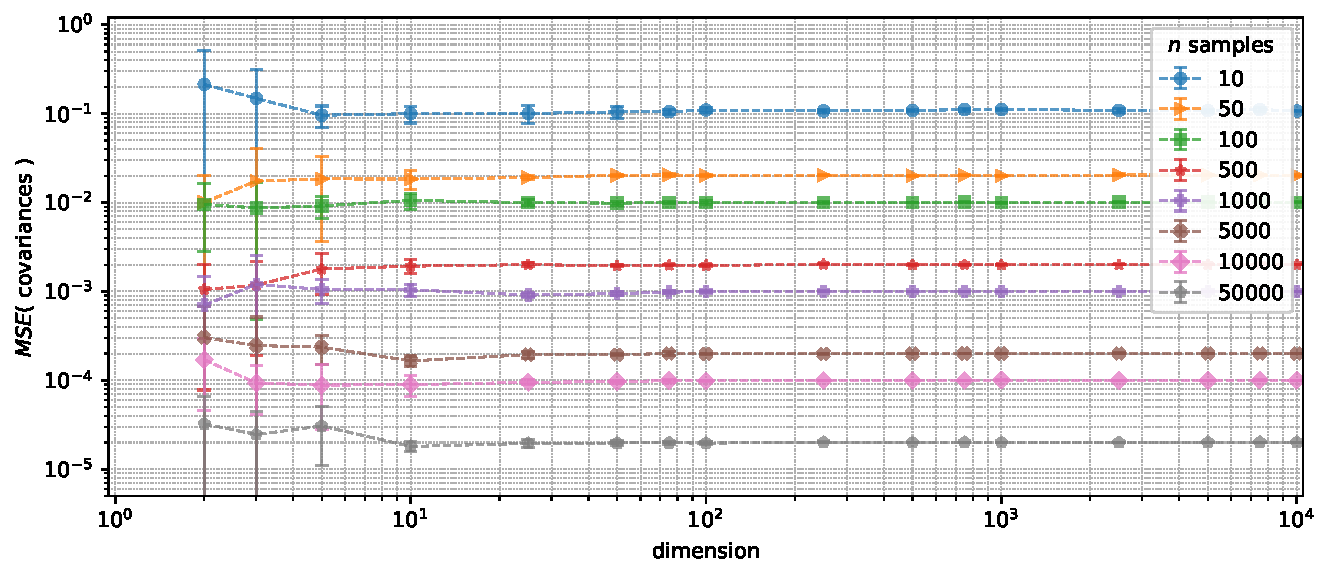
\includegraphics[width=\textwidth]{images/estimation/trend-properties-mse_covs(dimension)-n_correlated_0.20-covariance_0.20-samples_10,50,100,500,1000,5000,10000,50000-aggregated.pdf}
        \label{fig:estimation-covariances}
    \end{subfigure}

    \vspace{-0.5em}
    \caption{The estimation errors of selected cluster properties. The cluster contains $n$ samples of dimension $d$, generated from $G = MVN$ distribution with small fraction of features $f_{corr} = 0.2$ slightly correlated $g_{corr} = 0.2$. The more $n$ samples provided, the~more accurate estimation. The~results are aggregated for multiple generator seeds $\xi$ and displayed as averages with~error~bars~(standard deviation).}
    \label{fig:estimation}
    \vspace{-2.5em}
\end{figure}

\begin{figure}[t]
    % StreamLit settings: width=9, height=4
    % X: [0.95, 10500.00]
    % Y: [0,000005, 1.20]
    \centering
    \vspace{-0.5em}
    \begin{subfigure}[b]{0.9\textwidth}
        \centering
        \caption{\small Error estimating means}
        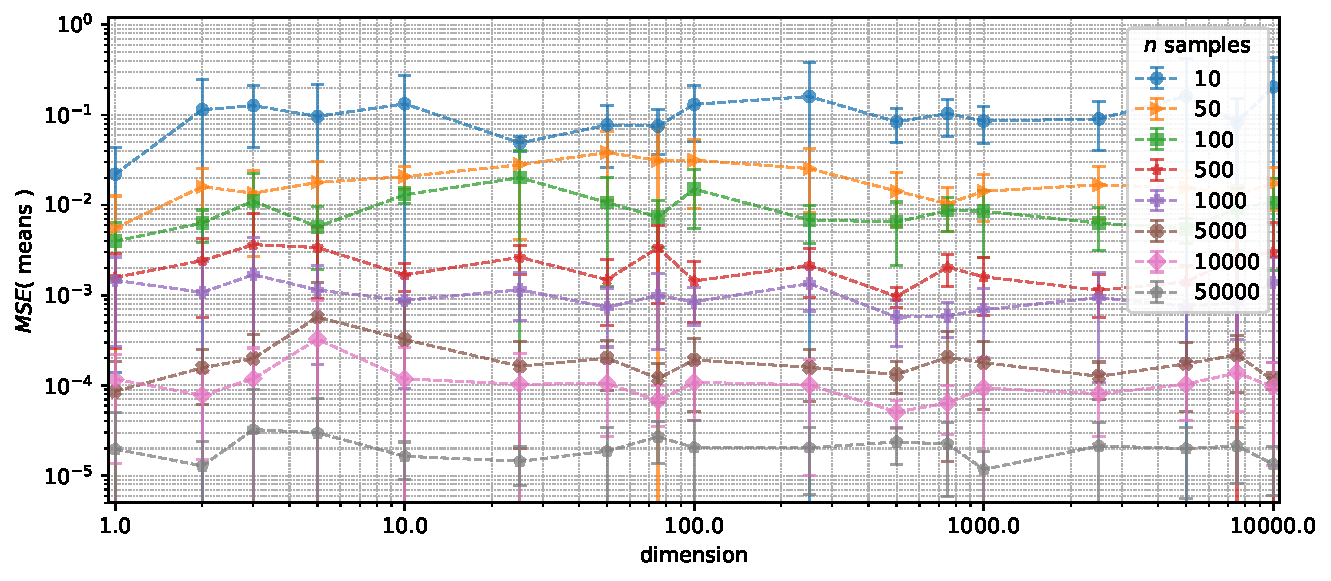
\includegraphics[width=\textwidth]{images/estimation/trend-properties-mse_means(dimension)-n_correlated_0.80-covariance_0.80-samples_10,50,100,500,1000,5000,10000,50000-aggregated.pdf}
        \label{fig:estimation-strong-means}
    \end{subfigure}

    \vspace{-0.5em}
    \begin{subfigure}[b]{0.9\textwidth}
        \centering
        \caption{\small Error estimating variances}
        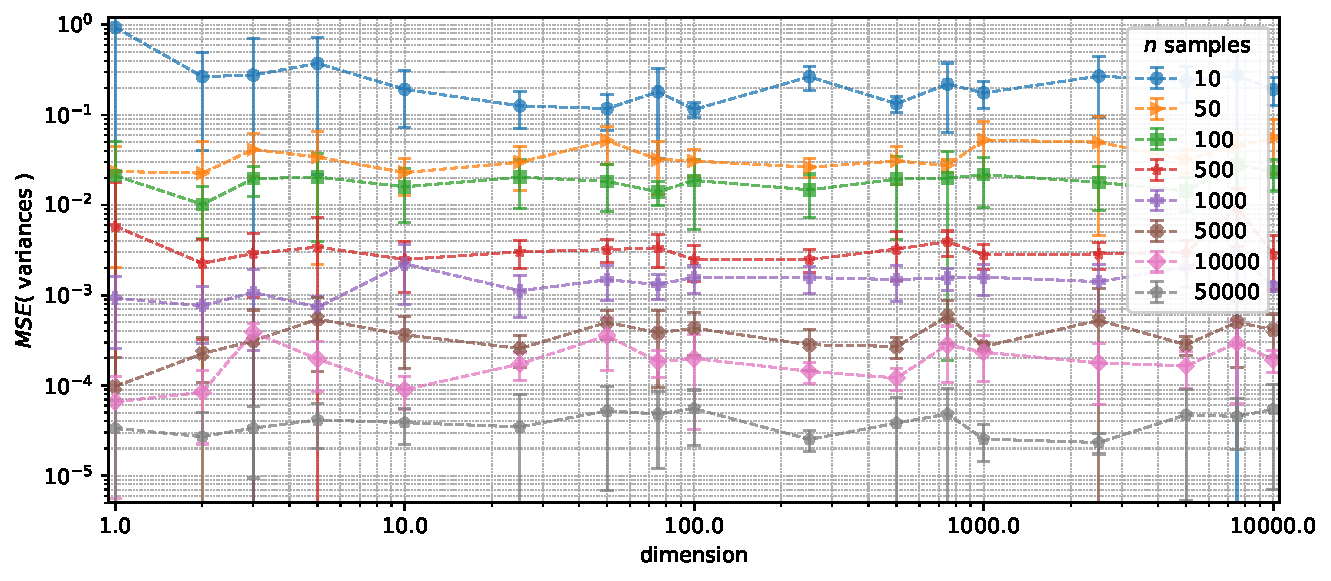
\includegraphics[width=\textwidth]{images/estimation/trend-properties-mse_vars(dimension)-n_correlated_0.80-covariance_0.80-samples_10,50,100,500,1000,5000,10000,50000-aggregated.pdf}
        \label{fig:estimation-strong-variances}
    \end{subfigure}

    \vspace{-0.5em}
    \begin{subfigure}[b]{0.9\textwidth}
        \centering
        \caption{\small Error estimating covariances}
        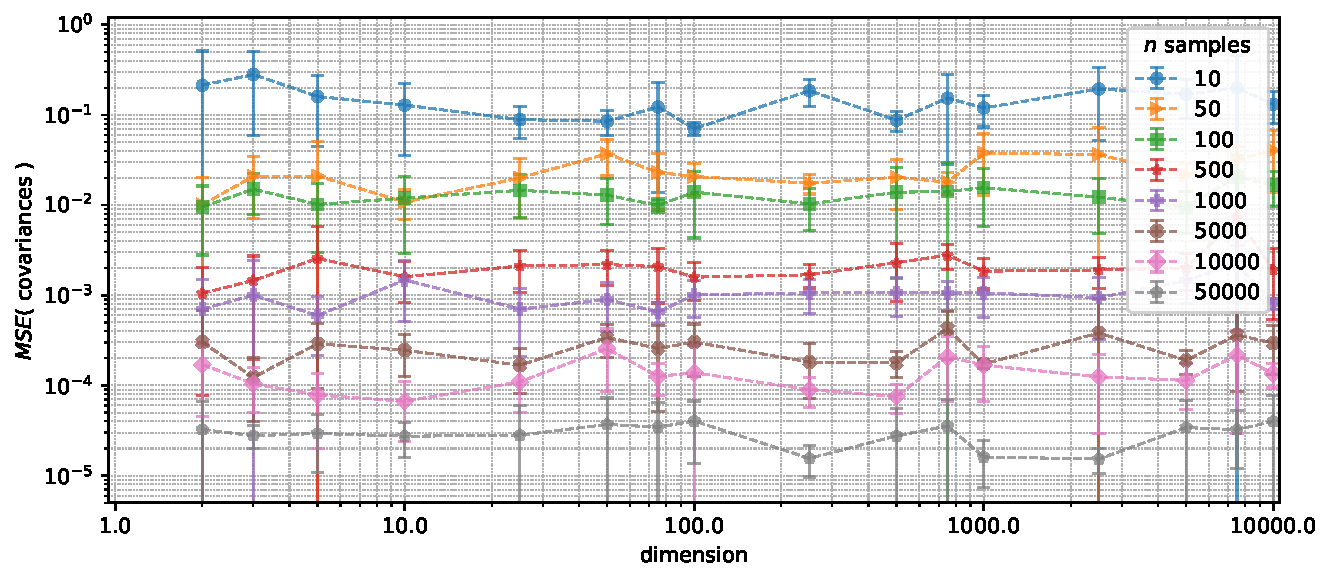
\includegraphics[width=\textwidth]{images/estimation/trend-properties-mse_covs(dimension)-n_correlated_0.80-covariance_0.80-samples_10,50,100,500,1000,5000,10000,50000-aggregated.pdf}
        \label{fig:estimation-strong-covariances}
    \end{subfigure}

    \vspace{-0.5em}
    \caption{The estimation errors of selected cluster properties. The cluster contains $n$ samples of dimension $d$, generated from $G = MVN$ distribution with great fraction of features $f_{corr} = 0.8$ highly correlated $g_{corr} = 0.8$. Under strong correlation, results are less stable, yet remaining of the same order. The~results are aggregated for multiple generator seeds $\xi$ and displayed as averages with~error~bars~(standard deviation).}
    \label{fig:estimation-strong}
    \vspace{-2.5em}
\end{figure}

\cleardoublepage{}
